

\newpage
\null 
\vfill
\begin{center}
\textbf{\large Ameer Muhammed (42843)}
\end{center}
\vfill
\fancyhead[L]{MNG GUI (Ameer Muhammed 42843)}
\clearpage	

\chapter{MNG GUI Part I}
\section{GUI Client Implementation}
\subsection{GUI Application Overview}
The graphical user interface (GUI) serves as the client-side control, monitoring, and visualization layer of the Measurement Network Gateway (MNG) system. Its core responsibility is to establish and manage a TCP connection to the measurement server, issue control and configuration commands, receive continuous streams of sensor data, and present this information to the user in real time.

Technically, the GUI integrates several subsystems that are typical of embedded-oriented monitoring applications. GTK is used for window management, layout, and event handling, POSIX sockets provide reliable network communication, pthreads enable concurrent execution, and the Cairo graphics library supports high-frequency, real-time signal visualization. These technologies are combined in a way that preserves responsiveness even when operating under sustained data rates.

A key architectural principle of the GUI is the strict separation between user interface execution and network communication. All GTK-related operations execute exclusively within the main thread, while network I/O and stream processing are delegated to a dedicated background thread. This separation ensures that blocking socket operations or transient network delays do not interfere with user interaction, window updates, or plotting performance.

In contrast to the server, which functions as a command-driven data producer governed by an internal streaming state machine, the GUI operates as a reactive consumer. User actions are translated into protocol-compliant control messages, while incoming binary sensor data is decoded, buffered, and rendered without influencing server timing or acquisition behavior. The GUI therefore maintains no control over data generation itself, but focuses on safe command issuance, visualization, and state consistency on the client side.

Overall, the GUI is designed to be lightweight, robust, and scalable. By avoiding tight coupling with server-side logic and by isolating potentially blocking operations from the graphical interface, the implementation remains stable and responsive across a wide range of sampling frequencies and operating conditions. Detailed descriptions of the internal threading model, networking behavior, state management, and data handling are presented in the following sections.

\subsection{GUI Architecture and Threading Model}
The GUI application follows a multi-threaded architecture built around GTK’s strictly single-threaded main loop. GTK enforces that all widget creation, modification, and rendering operations occur exclusively within the main thread. Any attempt to manipulate GTK objects from auxiliary threads results in undefined behavior and application instability. As a consequence, all blocking or long-running activities must be isolated from direct interaction with the graphical interface.

To satisfy this constraint, the GUI introduces a dedicated network receive thread whose sole responsibility is to handle TCP communication with the server. This thread performs blocking socket operations, parses incoming network payloads, and inserts decoded sensor samples into shared data structures. Crucially, it never accesses GTK widgets directly. Instead, all user interface updates are deferred to the GTK main loop using \texttt{g\_idle\_add()}, which schedules callbacks to be executed safely in the main thread context.

\begin{figure}[H]
    \centering 
    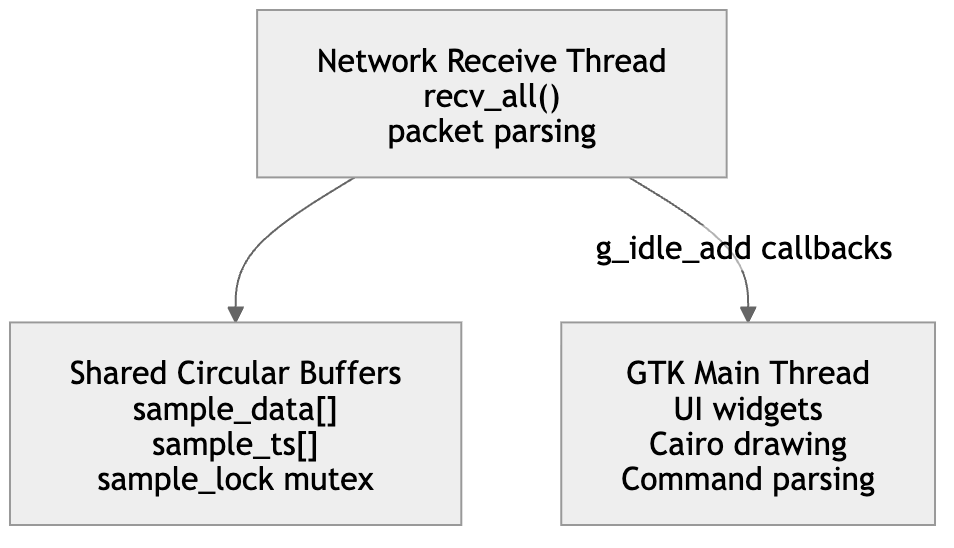
\includegraphics[scale = 0.5]{media/ameerapp9.png}
    \caption{GTK and Network Thread Separation}
    \label{fig-ameergui1}
\end{figure}

This design is reflected directly in the core synchronization primitives defined in the GUI implementation:

\begin{minted}[bgcolor = lightgray, fontsize = \footnotesize]{c}
static pthread_t net_thread;
static volatile int net_running = 0;

static pthread_mutex_t sample_lock = PTHREAD_MUTEX_INITIALIZER;
\end{minted}

The \texttt{net\_thread} executes the blocking receive loop, while the \texttt{net\_running} flag provides a lightweight, thread-safe termination mechanism used during disconnect and shutdown sequences. Shared access to sensor sample buffers is protected by \texttt{sample\_lock}, ensuring deterministic behavior when the network thread inserts new data and the GTK thread simultaneously renders plots or extracts values for display.

By isolating all network I/O inside a dedicated POSIX thread and strictly enforcing GTK-only access from the main loop, the architecture guarantees that user interactions such as window resizing, command entry, or sensor selection remain responsive regardless of network latency or streaming rate. This approach mirrors the separation of concerns used on the server side, where acquisition, communication, and scheduling responsibilities are similarly decoupled.

From a system-level perspective, the GUI therefore behaves as a reactive front-end: background threads ingest and buffer data, while the GTK main loop remains focused on deterministic rendering and user interaction.


\subsection{Socket Creation and Connection Establishment}
The connection workflow is initiated when the user provides a server IPv4 address and explicitly requests a connection through the GUI. At this point, the client creates a TCP socket using the Berkeley Sockets API and prepares it for controlled, non-blocking connection establishment. This approach ensures that the graphical interface remains responsive even when the remote server is unreachable or slow to accept connections.

To prevent the GUI from blocking during the \texttt{connect()} call, the
socket is temporarily configured in non-blocking mode. This allows the
application to initiate the connection asynchronously while retaining full
control over timeout behavior. The following excerpt illustrates the core
mechanism used during the connection phase:


\begin{minted}[bgcolor = lightgray, fontsize = \footnotesize]{c}
sock_fd = socket(AF_INET, SOCK_STREAM, 0);
fcntl(sock_fd, F_SETFL, O_NONBLOCK);

res = connect(sock_fd, (struct sockaddr *)&addr, sizeof(addr));
if (res < 0 && errno == EINPROGRESS)
{
    select(sock_fd + 1, NULL, &wfds, NULL, &timeout);
}
\end{minted}

In this configuration, \texttt{connect()} typically returns immediately with
\texttt{EINPROGRESS}, indicating that the connection attempt is still in
progress. The \texttt{select()} system call is then used to wait for the
socket to become writable within a bounded time interval. A three-second
timeout is applied to ensure deterministic behavior; if the socket does not
signal completion within this period, the connection attempt is aborted, the
socket is closed, and the user is notified via the GUI.

After \texttt{select()} returns, the connection result is verified using
\texttt{getsockopt()} with the \texttt{SO\_ERROR} option to distinguish a
successful connection from a failed attempt. Only if this check confirms
success does the GUI proceed to the next stage.

Once the connection attempt completes successfully, the socket is explicitly
restored to blocking mode. This design choice simplifies all subsequent
network operations: steady-state data reception is handled inside a dedicated
network receive thread, where blocking \texttt{recv()} calls provide
predictable control flow, reduced CPU usage, and eliminate the need for
polling or partial-read handling logic.

Immediately after restoring blocking mode, the GUI spawns the network receive
thread and transitions its internal state to indicate an active connection.
This staged strategy---non-blocking during connection establishment and
blocking during steady-state streaming---reflects common industrial client
implementations and achieves a balance between user-interface responsiveness
and reliable, low-complexity data handling.

\subsection{IPv4 Address Validation and Defensive Input Handling}
Before attempting any network operation, the GUI performs strict validation of the user-supplied IPv4 address. Instead of relying on permissive system-level parsing, the application enforces an exact dotted-decimal format consisting of four octets, each constrained to the valid range of 0 to 255.

This validation is executed locally within the GUI layer to prevent unnecessary socket creation attempts and to provide immediate, deterministic feedback to the user. Inputs containing missing octets, trailing characters, non-numeric tokens, or out-of-range values are explicitly rejected before any networking API is invoked.

The validation logic relies on strict pattern matching using sscanf(), ensuring that the input string contains exactly four numeric fields and no additional characters:
\begin{minted}[bgcolor = lightgray, fontsize = \footnotesize]{c}
if (sscanf(ip, "%d.%d.%d.%d%c", &a, &b, &c, &d, &tail) != 4)
    return FALSE;
\end{minted}

By rejecting malformed input at the earliest possible stage, the GUI avoids undefined behavior at lower networking layers and eliminates ambiguous error conditions that would otherwise surface during socket creation or connection attempts. This defensive approach improves both robustness and debuggability, particularly in failure scenarios involving invalid user input.

The outcome of the validation is immediately reflected in the graphical interface through dynamic visual feedback. The input field is styled to indicate success or error conditions, reinforcing correct usage patterns and reducing the likelihood of repeated invalid attempts. This tight integration of validation logic and UI feedback contributes to a safer and more user-friendly connection workflow.

\subsection{GUI State Machine Design}
The GUI implements an internal client-side state machine that is intentionally
distinct from the server's streaming state machine. While the server operates
using internal states such as \texttt{STREAM\_IDLE}, \texttt{STREAM\_RUNNING},
and \texttt{STREAM\_DISCONNECT} to manage data production and transmission,
the GUI maintains a higher-level, connection-oriented view of system
operation. This separation ensures that client-side logic remains focused on
user interaction, command validity, and visualization control rather than
internal server behavior.

From the GUI's perspective, system operation is fully characterized by three
states. In the disconnected state, no TCP connection exists and all
network-related actions are disabled. The connected state represents a
successfully established TCP connection in which the system is ready to accept
user commands but is not yet receiving streaming data. The running state
indicates that real-time sensor data streaming is active and being processed
and visualized by the GUI.


\begin{figure}[H]
    \centering 
    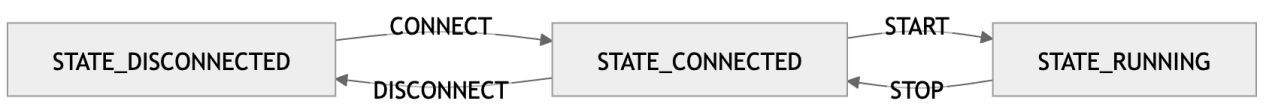
\includegraphics[scale = 0.9]{media/ameerapp10.png}
    \caption{Client Connection State Machine}
    \label{fig-ameergui2}
\end{figure}

State transitions are strictly validated before execution to prevent illegal command sequences and unsafe operations. For example, streaming can only be initiated when the GUI is already connected, and disconnection is explicitly blocked while streaming is active. The following excerpt illustrates a guarded transition from the connected state into the running state when the user issues a valid START command:

\begin{minted}[bgcolor = lightgray, fontsize = \footnotesize]{c}
if (state == STATE_CONNECTED) {
    send(sock_fd, "START\n", 6, 0);
    state = STATE_RUNNING;
}
\end{minted}
By enforcing these constraints locally, the GUI acts as a first line of defense against invalid protocol usage. This prevents malformed or out-of-sequence commands from reaching the server and ensures that the graphical controls, internal logic, and remote system remain synchronized at all times.

\subsection{Network Receive Thread and Streaming Handling}
Once streaming is initiated, the GUI spawns a dedicated network receive thread that becomes the sole entry point for incoming data from the measurement server. This thread is intentionally isolated from all GTK operations and performs blocking socket I/O, allowing the main GUI thread to remain fully responsive during high-rate data transfers.

The server transmits sensor data using a length-prefixed framing scheme. Each transmission begins with a fixed 4-byte header indicating the size of the upcoming payload, followed by a contiguous batch of binary \texttt{sensor\_data\_t }records. Since TCP is a stream-oriented protocol with no inherent message boundaries, this framing mechanism is essential to preserve packet alignment and ensure deterministic decoding on the client side.

The receive thread first blocks until the size header is fully received, converts it from network byte order, and then continues reading until the complete payload has been transferred. This logic is implemented using a helper routine that guarantees full reception before processing:
\begin{minted}[bgcolor = lightgray, fontsize = \footnotesize]{c}
recv_all(sock_fd, &net_size, sizeof(net_size));
payload_size = ntohl(net_size);
recv_all(sock_fd, batch, payload_size);
\end{minted}

To support this behavior, a blocking helper function repeatedly invokes \texttt{recv()} until the requested number of bytes has been obtained or an error occurs:

\begin{minted}[bgcolor = lightgray, fontsize = \footnotesize]{c}
static int recv_all(int fd, void *buf, size_t len)
{
    size_t off = 0;
    while (off < len)
    {
        ssize_t n = recv(fd, (char *)buf + off, len - off, 0);
        if (n <= 0)
            return -1;
        off += n;
    }
    return 0;
}
\end{minted}

This approach eliminates partial-read corner cases and ensures that each batch is processed atomically. Once the payload has been successfully received, the thread iterates through the decoded sensor records and forwards them to the circular buffer layer via the \texttt{push\_sample()} interface.

\begin{figure}[H]
    \centering 
    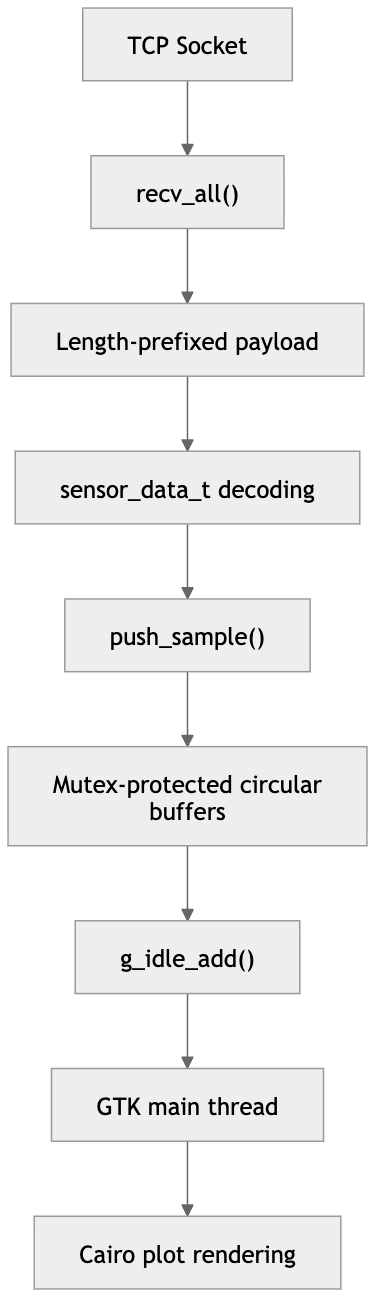
\includegraphics[scale = 0.7]{media/ameerapp2.png}
    \caption{Client-Side Data Flow Pipeline}
    \label{fig-ameergui2}
\end{figure}

Crucially, the receive thread never updates GUI elements directly. Instead, it schedules redraw operations and auxiliary UI updates using \texttt{g\_idle\_add()}, which defers execution to the GTK main loop. This design strictly adheres to GTK’s thread-safety model and prevents undefined behavior caused by cross-thread widget access.
 
In the event of a socket error, malformed payload, or remote disconnect, the receive loop terminates gracefully. The thread then signals the main thread to reset the plotting state, close the socket, and transition the GUI back into a disconnected state. This controlled shutdown sequence ensures that resources are released safely and that the application never remains in an inconsistent or partially connected condition.

\subsection{Circular Buffer Handling and Sample Insertion}
Incoming sensor samples received by the network thread are stored in fixed-size circular buffers, one buffer per sensor. Each buffer maintains its own head index and sample counter, allowing the GUI to retain only the most recent data while guaranteeing bounded memory usage regardless of streaming duration.

All write access to the buffers is protected by a POSIX mutex (sample\_lock). This ensures that concurrent access from the network receive thread and the GTK rendering logic does not result in race conditions or inconsistent state.

The core insertion mechanism follows a deterministic overwrite model. Each new sample is written at the current head position, after which the head index is advanced with wraparound logic:
\begin{minted}[bgcolor = lightgray, fontsize = \footnotesize]{c}
pthread_mutex_lock(&sample_lock);

sample_data[sid][head] = value;
sample_ts[sid][head]   = rel_ts;

sample_head[sid] = (head + 1) % MAX_SAMPLES;

if (sample_count[sid] < MAX_SAMPLES)
    sample_count[sid]++;

pthread_mutex_unlock(&sample_lock);
\end{minted}

This approach ensures that once the buffer reaches capacity, older samples are automatically overwritten by newer ones in a predictable manner. No dynamic memory allocation occurs during steady-state operation, which is essential for maintaining consistent performance under high-frequency data acquisition.

A key design element is timestamp normalization. The GUI establishes a reference timestamp (server\_t0) when the first sample is received. All subsequent timestamps are stored as offsets relative to this reference:


\begin{minted}[bgcolor = lightgray, fontsize = \footnotesize]{c}
if (server_t0 == 0)
    server_t0 = ts;

uint64_t rel_ts = ts - server_t0;
\end{minted}

This normalization simplifies later visualization and axis scaling by eliminating large absolute timestamp values and ensuring that all plotted data shares a common temporal origin. It also allows the GUI to reset its time base cleanly whenever a new connection or streaming session begins.

The circular buffers therefore serve as a stable synchronization boundary between asynchronous data ingestion and deterministic GUI rendering, enabling smooth real-time visualization without unbounded memory growth.

\subsection{GUI–Network Interaction Model}
Direct interaction between background threads and GTK widgets is strictly prohibited in the application design. GTK enforces a single-threaded UI model in which all widget updates, rendering operations, and state changes must occur within the main GTK thread. Violating this rule can lead to race conditions, segmentation faults, or undefined rendering behavior. As a result, the GUI–network interaction is implemented using a strictly event-driven synchronization mechanism.

The network receive thread is therefore designed to operate in complete isolation from the GUI layer. Its responsibilities are limited to blocking socket I/O, decoding incoming protocol messages, and inserting validated sensor samples into mutex-protected circular buffers. At no point does this thread directly invoke GTK drawing routines or manipulate widget state.

To bridge the gap between background processing and UI updates, the GUI leverages GTK’s idle event mechanism. Whenever new data arrives or a state transition must be reflected visually, the network thread schedules a deferred callback using \texttt{g\_idle\_add()}. This registers a lightweight task that is executed asynchronously by the GTK main loop when it reaches an idle state.

\begin{minted}[bgcolor = lightgray, fontsize = \footnotesize]{c}
g_idle_add((GSourceFunc)gtk_widget_queue_draw, graph_area);
\end{minted}

This approach guarantees that all rendering activity, including plot redraws and widget refreshes, is executed safely within the GTK thread context. The same mechanism is reused for non-graphical updates, such as appending entries to the live sensor information panel or updating connection status labels following network events.

By enforcing a unidirectional interaction model—where background threads publish events and the GUI consumes them—the implementation achieves strong temporal decoupling between data acquisition and visualization. This design not only preserves thread safety but also ensures that GUI responsiveness is unaffected by network latency, bursty data arrival, or temporary connection instability.

The event-driven interaction model thus forms a critical stability boundary within the client architecture. It allows high-frequency sensor streaming to coexist with a responsive graphical interface, while maintaining strict compliance with GTK’s threading constraints.

\subsection{GUI Utility Layer}
The GUI utility layer provides a compact collection of shared helper functions and data structures that support the main GUI logic without embedding auxiliary concerns directly into gui.c. Its primary role is to centralize functionality that is reused across multiple GUI subsystems, thereby improving code clarity, maintainability, and separation of concerns.

At the functional level, the utility layer encapsulates three main responsibilities: defensive input validation, lightweight widget state management, and consistent visual feedback through runtime CSS injection. By isolating these tasks, the core GUI implementation remains focused on application logic, networking, and visualization rather than low-level UI mechanics.

A key example is IPv4 address validation, which is implemented once in the utility layer and reused by both button-driven and CLI-driven connection workflows. This avoids duplicated validation logic and ensures consistent behavior regardless of how a connection is initiated.
\begin{minted}[bgcolor = lightgray, fontsize = \footnotesize]{c}
gboolean is_valid_ipv4(const char *ip)
{
    int a, b, c, d;
    char tail;
    if (sscanf(ip, "%d.%d.%d.%d%c", &a, &b, &c, &d, &tail) != 4)
        return FALSE;
    return (a >= 0 && a <= 255 &&
            b >= 0 && b <= 255 &&
            c >= 0 && c <= 255 &&
            d >= 0 && d <= 255);
}
\end{minted}

In addition to validation helpers, the utility layer defines the shared data structures that form the binary protocol contract between the GUI client and the server. These structures are intentionally placed in \texttt{utils.h} to guarantee that both networking code and visualization logic operate on a common, unambiguous data model.

\begin{minted}[bgcolor = lightgray, fontsize = \footnotesize]{c}
typedef struct
{
    sensor_id_t sensor_id;
    unsigned int sensor_value;
    uint64_t timestamp;
} sensor_data_t;

typedef struct
{
    sensor_rate_t rates[SENSOR_COUNT];
} RatesMsg;
\end{minted}

The \texttt{sensor\_data\_t} structure represents a single atomic sensor sample transmitted by the server, while RatesMsg encapsulates the sampling configuration exchanged at the start of streaming. Together, these definitions ensure binary compatibility between the server’s transmit logic and the GUI’s receive and decode paths, reducing the risk of protocol mismatches.
Finally, the utility layer manages GUI-specific presentation details such as command feedback styling. Custom CSS rules are injected at runtime to visually distinguish successful commands, invalid input, and focus transitions, without hard-coding presentation logic into widget callbacks.

\begin{minted}[bgcolor = lightgray, fontsize = \footnotesize]{c}
gtk_css_provider_load_from_data(provider,
    "entry.cmd-success { border: 2px solid #2ecc71; }"
    "entry.cmd-error   { border: 2px solid #e74c3c; }",
    -1, NULL);
\end{minted}

By confining these responsibilities to a dedicated utility module, the GUI implementation achieves a cleaner architectural structure. The result is a client application that is easier to extend, debug, and reason about, while preserving a clear boundary between core behavior and supporting infrastructure.

\subsection{Summary and Observations}
The GUI client implementation provides a stable and efficient front-end for interacting with the Measurement Network Gateway under real-time operating conditions. By separating graphical operations from network communication and enforcing strict execution boundaries between threads, the design maintains responsiveness even during high-frequency data streaming.

A dedicated network receive thread, combined with mutex-protected circular buffers and GTK’s idle-event scheduling, ensures safe and deterministic data flow from the TCP socket to the visualization layer. Defensive IPv4 validation and a clearly defined client-side state machine prevent invalid command sequences and maintain consistency between user actions, GUI controls, and server behavior.

Overall, the GUI complements the server architecture by offering a scalable, robust, and user-oriented interface for real-time measurement monitoring, while adhering to sound systems programming practices suitable for high-throughput embedded and networked applications.




\clearpage 
\null 
\vfill 
\begin{center}
\textbf{\large Haizon Helet Cruz (42708)}
\end{center}
\vfill 
\fancyhead[L]{MNG GUI (Haizon Helet Cruz 42708)}
\clearpage


\chapter{MNG GUI Part II}
\section{GUI PLOTTING}
This section handles the plotting of the graph for individual sensors which are sent from the network thread. This is a framed drawing area for live plotting using \texttt{gtk\_frame\_new}, which creates a \texttt{GtkFrame} container and the string ``Plot'' becomes the visible title of the frame. The section is set to expand the window vertically when the window resizes.

The drawing area is created using \texttt{gtk\_drawing\_area\_new} which renders a blank canvas and the graph is drawn using the Cairo library. The canvas is supposed to occupy the whole of section B, even in cases where the window resizes. Then this plot is connected to corresponding functions \texttt{draw\_grid}, \texttt{gtk\_widget\_queue\_draw}, \texttt{update\_info\_text\_colors}, which are used to render the graph. This section also includes the text box which displays the last 10 values of temperature and ADC.

\subsection{DATA FLOW}
Incoming sensor information is organized into a dedicated circular buffer managed by the \texttt{push\_sample()} function. Each individual sensor maintains a structured dataset consisting of \texttt{id}, \texttt{value} and \texttt{timestamp} defined as a struct named \texttt{sensor\_data\_t}. These buffers are designed to accommodate required data for the purpose of plotting. To maintain integrity and prevent data collisions during concurrent operations, a synchronization mechanism utilizes mutex. This lock regulates all access to the shared sample buffers, ensuring that the ingestion of new packets occurs in a thread-safe manner. By acquiring this mutex before any modification to the circular arrays, the system prevents race conditions and guarantees that the internal state of the sensor data remains consistent and reliable for any process attempting to read or write to the memory.

The architecture maintains a clean separation between data ingestion and the user interface to ensure overall stability. Background processes are prohibited from directly modifying graphical elements instead the \texttt{g\_idle\_add} is used to schedule necessary updates. This approach delegates all rendering tasks to the GTK main thread, ensuring that the GUI remains responsive and that all visual modifications are executed within the correct execution context.

The visualization employs a dynamic windowing strategy to ensure that only the most relevant sensor data is rendered on screen. By identifying the most recent timestamp across all active sensors denoted as \texttt{t\_max}, the GUI plot establishes a temporal anchor for the display. A lower boundary \texttt{t\_min}, is then calculated using the formula \texttt{t\_min = t\_max - time\_window\_us}. During the rendering phase, any samples with timestamps failing outside this range are clipped, ensuring the graph remains focused on the current activity and prevents visual clutter from stable data. The duration of this visible window, defined by \texttt{time\_window\_us}, is not static but scales intelligently based on the incoming sampling frequency. This is particularly critical for high rate sources like ADC0, where the window must balance detail with performance.

\subsection{COORDINATE TRANSFORMATION AND SIGNAL NORMALIZATION}
Once the visible time interval is determined through the dynamic windowing
mechanism, each valid sample must be transformed from data-space into
screen-space coordinates. This conversion is performed during the rendering
phase inside the Cairo draw callback. The horizontal coordinate is calculated
by linearly mapping each timestamp within the interval $[t_{min}, t_{max}]$
to the available plotting width. This ensures that the leftmost edge of the
graph corresponds to the beginning of the visible time window, while the
rightmost edge reflects the most recent data sample.

The vertical coordinate is computed using a normalization strategy that allows
multiple sensors to be plotted simultaneously on a unified scale, Since
different sensors operate over different numeric ranges, each sensor is
associated with a defined maximum range in the array
\texttt{sensor\_y\_\_max}. During rendering, raw values are divided by their
respective maximums to obtain a normalized ratio between 0 and 1. This ratio
is then scaled to the height of the plotting region. Clamping is applied where
necessary to prevent graphical overflow. This approach simplifies comparative
visualization and maintains consistent scaling across multiple sensor types
without requiring dynamic axis configuration.

\subsection{GRID, AXES and TICK CONSTRUCTION}
To improve interpretability, the plotting system renders a structured
background consisting of grid lines, axes, tick marks and axis labels. The
grid is drawn first using faint, semi-transparent lines to provide spatial
reference without overpowering the sensor traces. Vertical grid lines
correspond to grid progression, while horizontal grid lines represent
normalized value increments. The axes are rendered with greater line thickness
to distinguish them from the grid. Directional arrows are added to both axes
to indicate increasing time and increasing signal magnitude. Tick marks are
placed at uniform pixel intervals, and corresponding numeric labels are
computed dynamically. For the X-axis, timestamps are converted to milliseconds
and formatted to avoid excessive digit length, reducing visual clutter, The
Y-axis labels reflect normalized values within the $0$--$1$ range. Axis titles
are rendered with appropriate font scaling and positioning. THe Y-axis title
is rotated vertically using the Cairo transformation matrix, ensuring
conventional scientific plot orientation.

\subsection{MULTI-SENSOR RENDERING AND TRACE STYLING}
The plotting subsystem supports simultaneous visualization of up to two
sensors. This constraint is enforced at the user interface level to maintain
clarity and prevent excessive graphical overlap. During each redraw cycle, the
renderer iterates through the selected sensors and extracts only the samples
that fell within the active window.

For each sensor, a continuous line trace is drawn by sequentially connecting
visible samples. Cairo path operations are used to move to the first valid
coordinate and then draw line segments to subsequent points. Each sensor trace
is assigned a distinct color selected from a predefined palette to ensure
clear differentiation. Line thickness is increased slightly relative to the
grid lines to enhance visibility. By decoupling the rendering logic from the
packet arrival rate and instead relying on periodic redraw scheduling, the
system ensures that trace updates remain smooth and consistent even under
high-frequency sampling conditions.


\subsection{DYNAMIC LEGEND RENDERING AND THEME ADAPTION}
To aid interpretation, a dynamic legend is rendered directly within the
plotting area. The legend displays only the currently selected sensors and
includes a colored marker alongside each sensor label. The dimensions of the
legend box are computed at runtime based on the width of the text elements,
ensuring that the container adapts automatically to varying content. The
legend background color is not statically defined. Instead, the GUI retrieves
the active GTK theme colors and performs luminance analysis to adjust the
legend background for sufficient contrast. In darker themes, the background is
slightly lightened while in lighter themes it is subtly darkened. This
guarantees readability regardless of the user's selected interface theme.
Additionally, style update signals trigger automatic redraws when the GTK
theme changes, maintaining visual consistency.

\begin{figure}[H]
\centering 
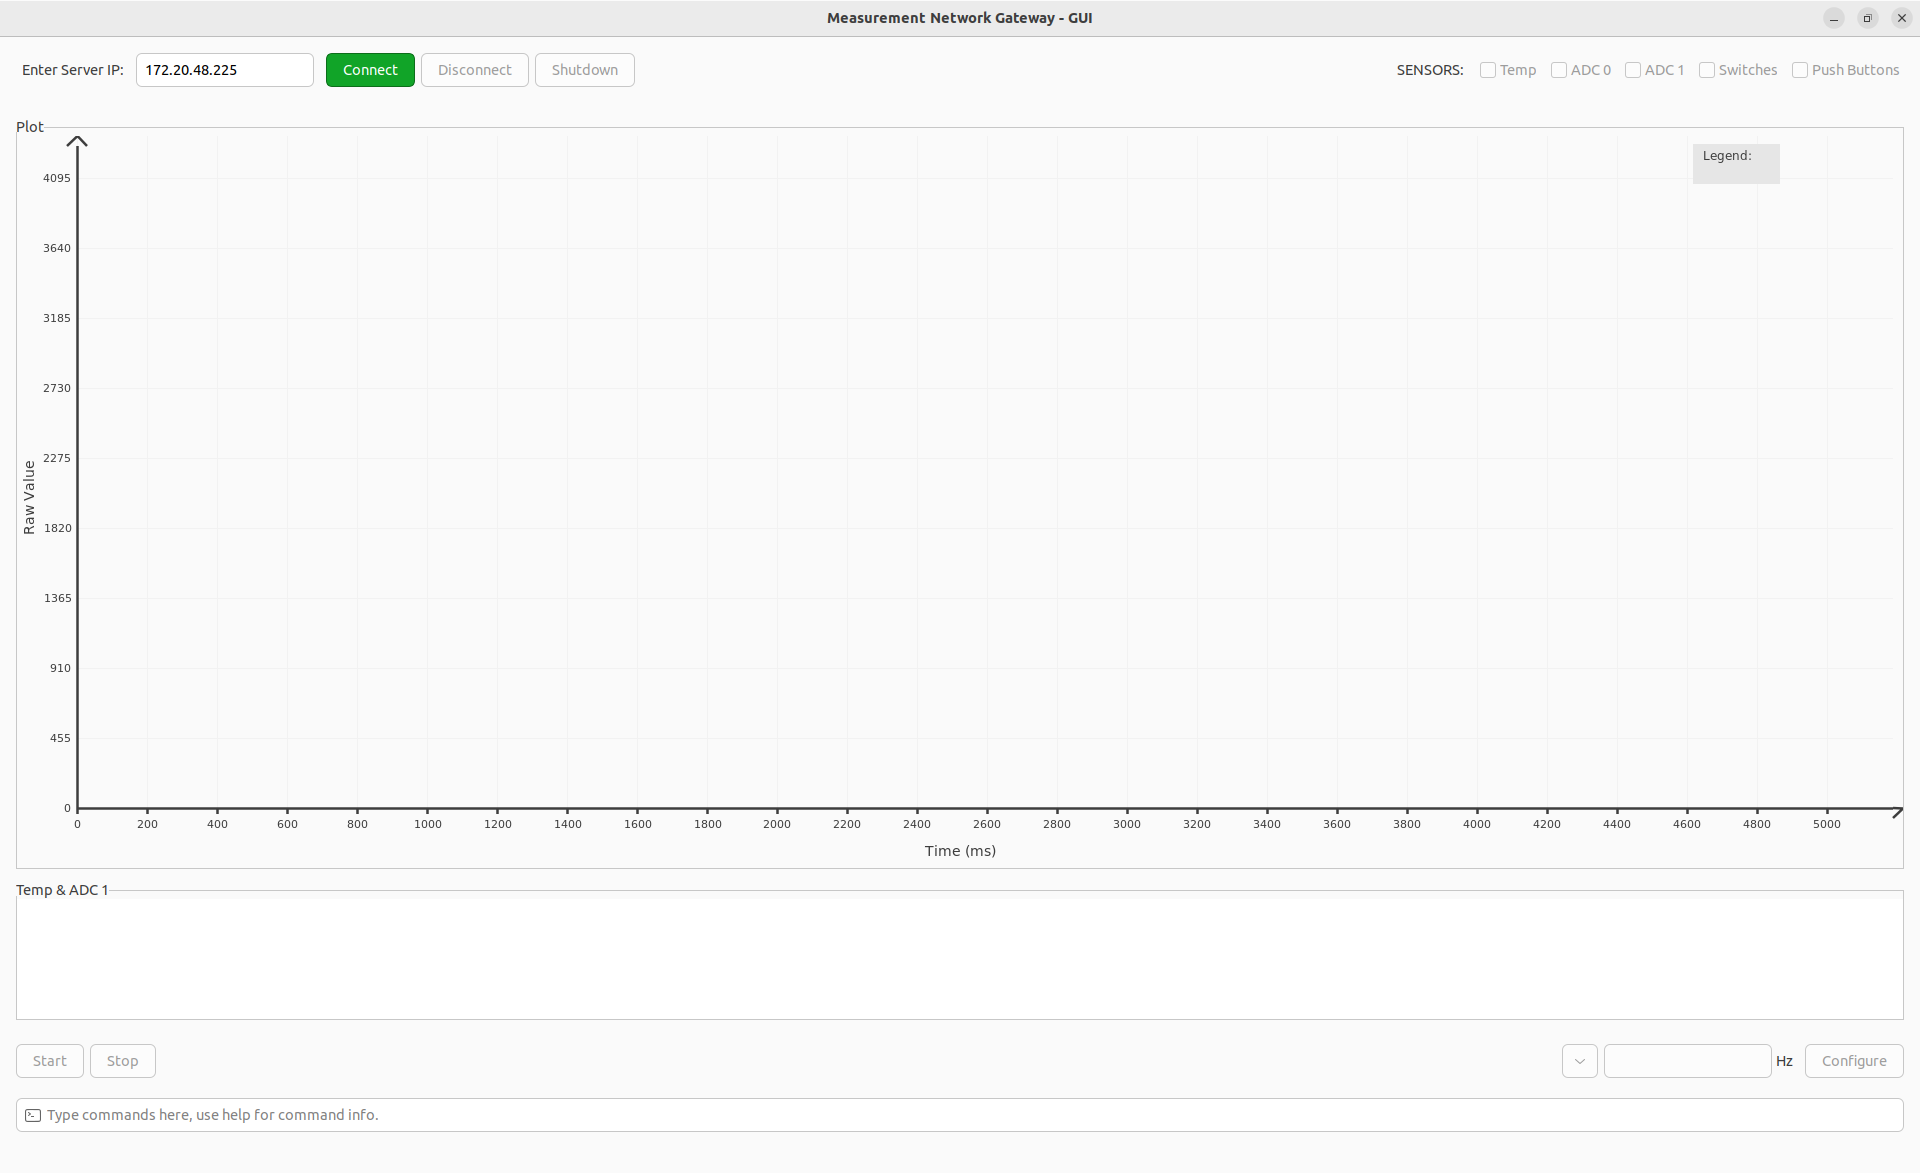
\includegraphics[width = \textwidth]{media/guihaa5.png}
\label{fig-guihaa5}
\end{figure}

\begin{figure}[H]
\centering 
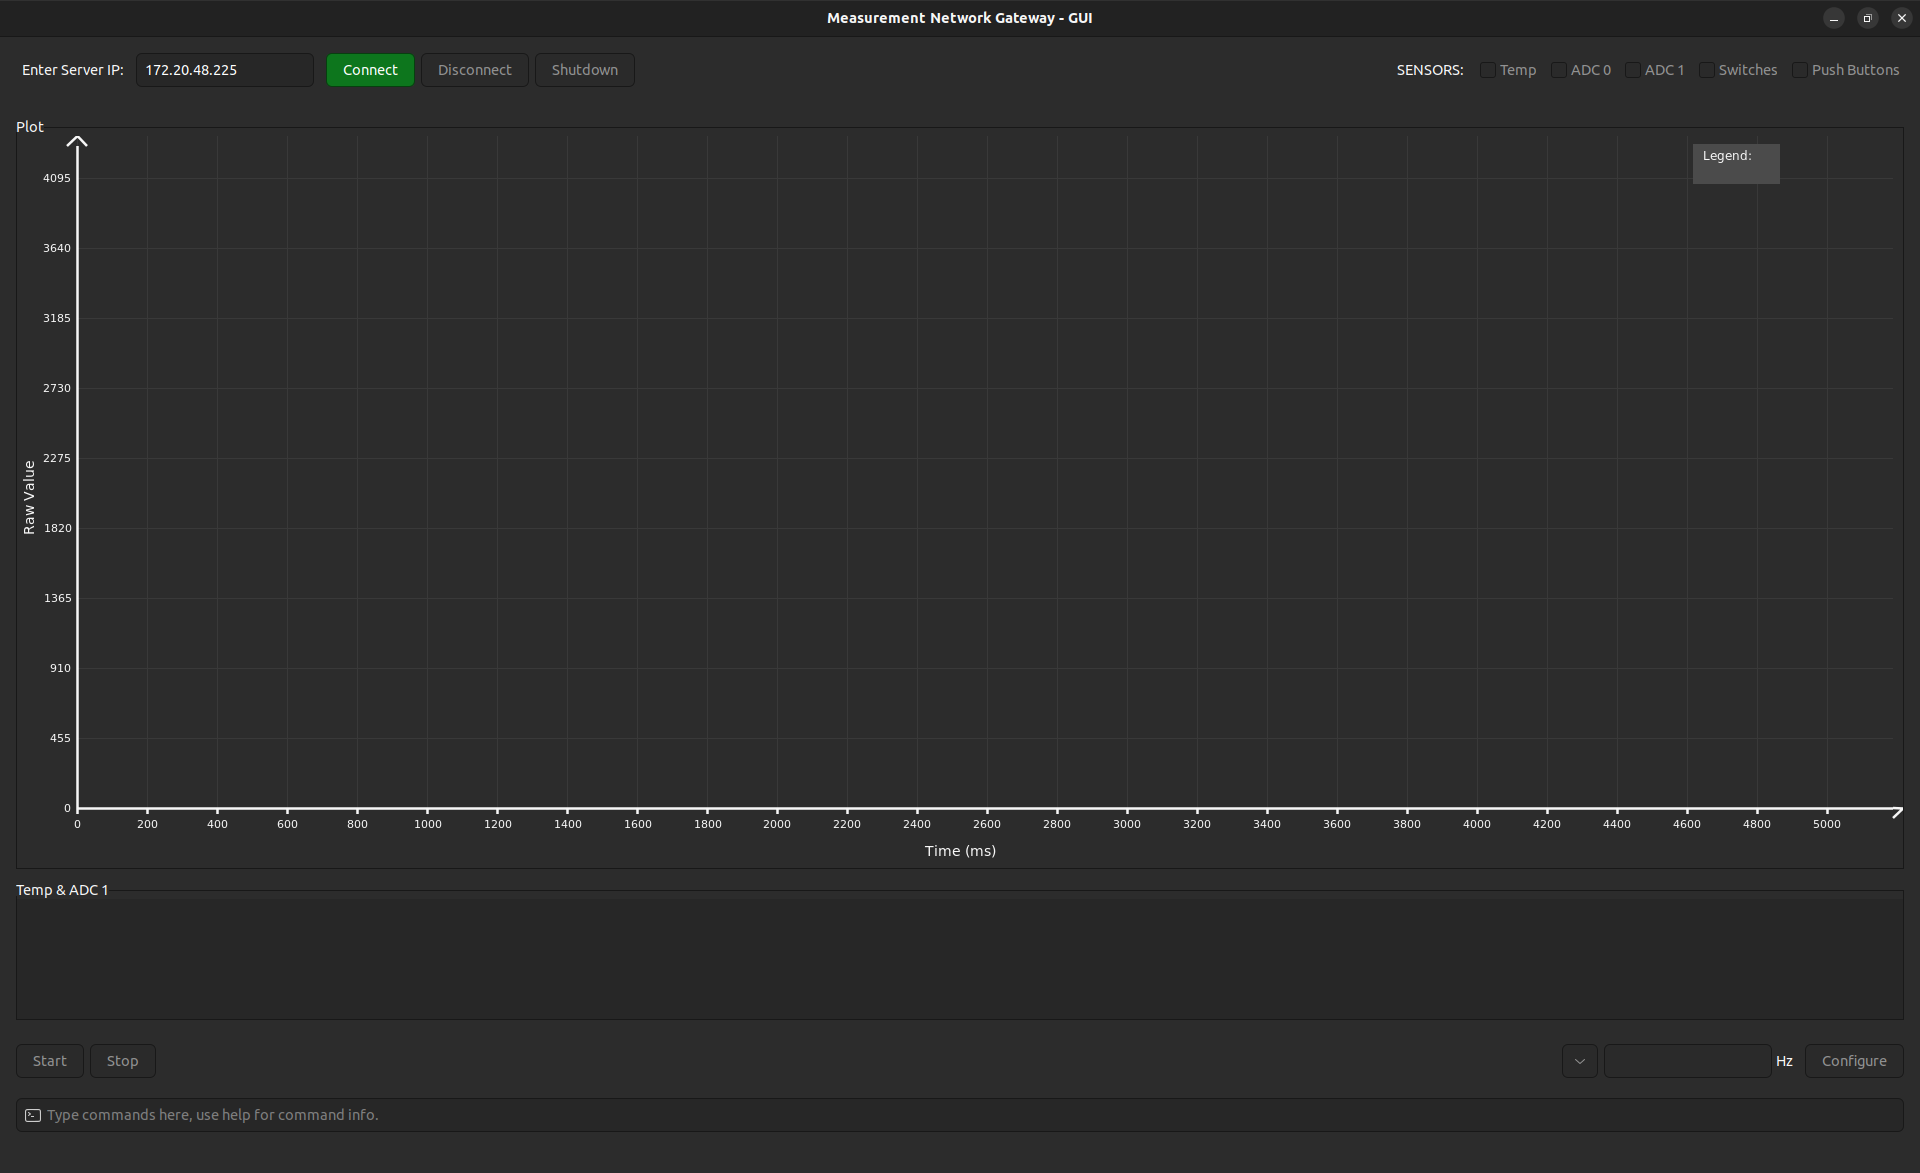
\includegraphics[width = \textwidth]{media/guihaa6.png}
\label{fig-guihaa6}
\end{figure}

\clearpage 
\section{Redraw Strategy and Performance Consideration}
Rather than redrawing the plot upon every incoming sample, the application
employs a timed refresh mechanism using a 33-millisecond interval. This
corresponds to approximately 30 frames per second, which provides visually
smooth updates while limiting unnecessary computational load. The use of
circular buffers further enhances performance by preventing unbounded memory
growth and eliminating the need for dynamic memory allocation during plotting
operation. This design ensures that rendering workload remains predictable and
stable even when sensors operate at higher sampling frequencies. By separating
data acquisition, buffering, and visualization into distinct functional layers,
the architecture maintains responsiveness and scalability.

\begin{figure}[H]
\centering 
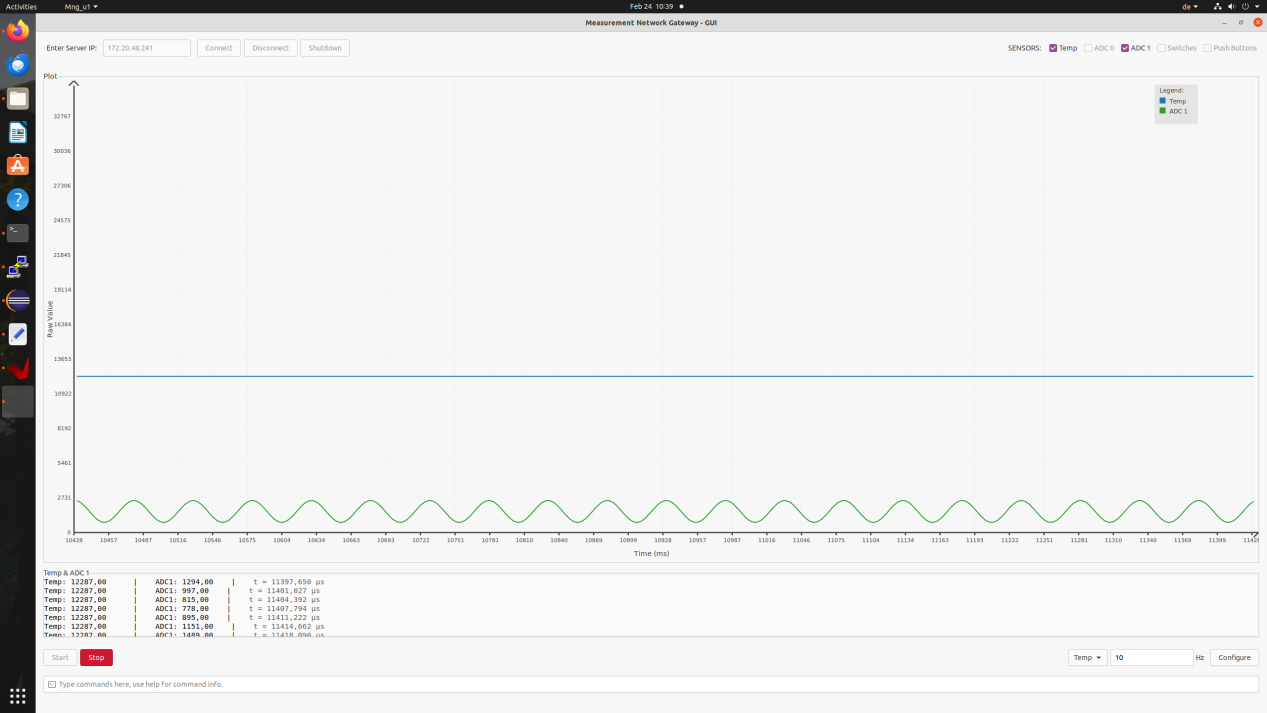
\includegraphics[width = \textwidth]{media/guihaa7.png}
\label{fig-guihaa7}
\end{figure}

\begin{figure}[H]
\centering 
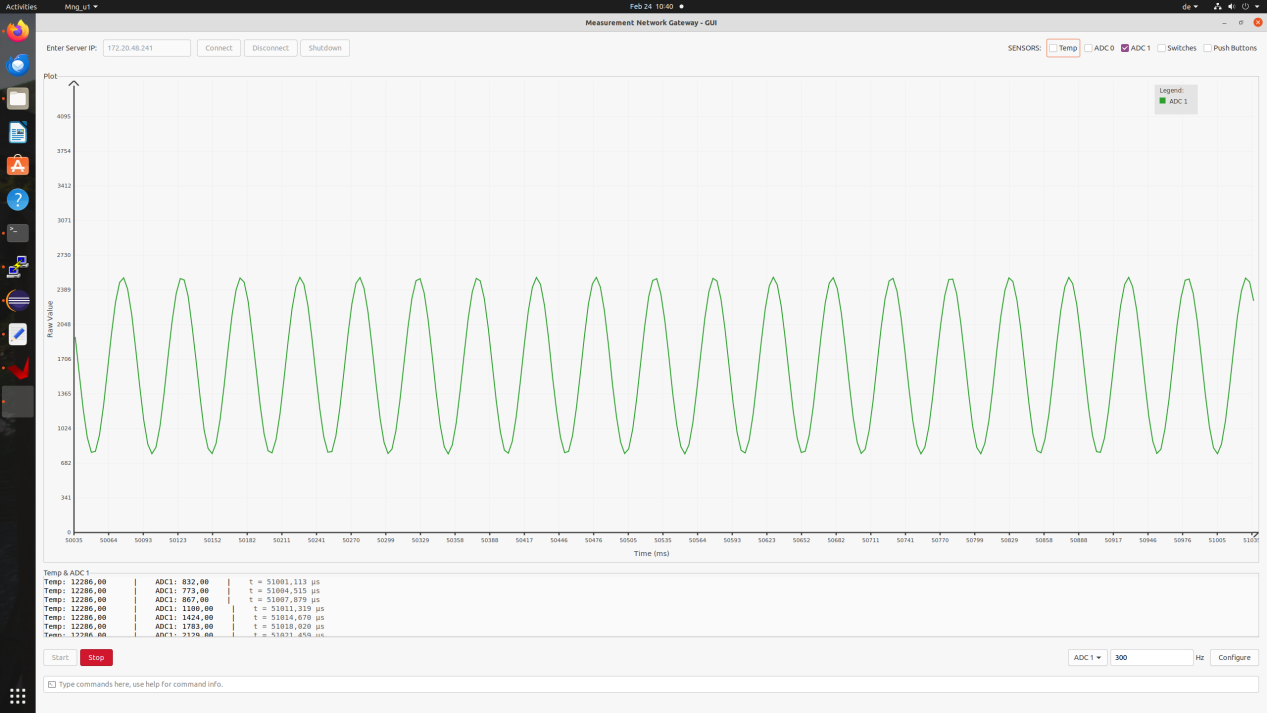
\includegraphics[width = \textwidth]{media/guihaa8.png}
\label{fig-guihaa8}
\end{figure}

\section{Live Sensor Information Panel}
Complementing the graphical plot, the interface includes a textual information
panel positioned below the main drawing area. This component displays the ten
most recent temperature and ADC1 measurements along with their corresponding
timestamps. The monospace font preserves column alignment. Whenever a new ADC1
sample is received, a formatted entry containing temperature, converted ADC
voltage, and relative timestamp is appended to the buffer. If the number of
lines exceeds 10, the oldest entry is automatically removed to maintain a
fixed-length history. Text tags are used to apply consistent color styling to
different data fields, enhancing readability. This panel serves as a numerical
complement to the graphical representation, allowing users to inspect precise
values while simultaneously observing real-time trends in the plot.

\begin{figure}[H]
\centering 
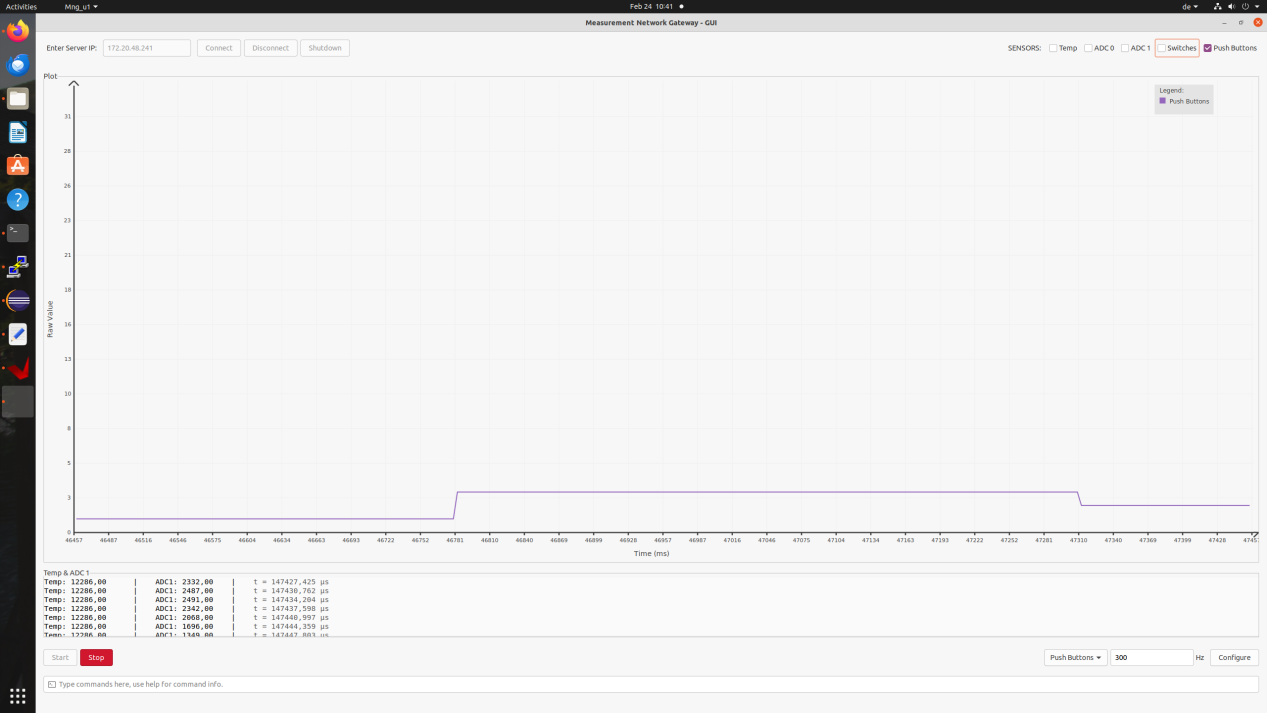
\includegraphics[width = \textwidth]{media/guihaa9.png}
\label{fig-guihaa9}
\end{figure}

\section{Command Line Interface}
The application includes an integrated command-line interface (CLI) help system
that provides structured guidance for all supported textual commands. When the
user enters the \texttt{HELP} command, a dedicated terminal window is launched
displaying a formatted reference guide. This help interface clearly categorizes
valid commands, usage syntax, parameter requirements, example invocations,
invalid usage scenarios, and operational constraints. The terminal output uses
visual formatting to distinguish command keywords, examples, warnings, and
notes, thereby improving readability and reducing user error.

The CLI supports core operational commands including \texttt{CONNECT},
\texttt{DISCONNECT}, \texttt{START}, \texttt{STOP}, \texttt{SHUTDOWN}, and
\texttt{CONFIGURE}. The \texttt{CONNECT <IP\_ADDRESS>} command establishes a
TCP connection to a remote measurement server, requiring a valid IPv4 address
in strict dotted-decimal format. The \texttt{DISCONNECT} command safely closes
an active connection but enforces a precondition that data streaming must be
stopped. The \texttt{START} command initiates sensor data streaming and
real-time plotting, and is valid only when a connection is active. Conversely,
the \texttt{STOP} command halts streaming and plotting and is permitted only
while the system is in a running state. The \texttt{SHUTDOWN} command instructs
the remote device to terminate operation and closes the application, provided
that streaming is not currently active.

The \texttt{CONFIGURE <SENSOR\_ID> <FREQ\_HZ>} command allows runtime
adjustment of individual sensor sampling frequencies. Supported sensor
identifiers include \texttt{TEMP}, \texttt{ADC0}, \texttt{ADC1}, \texttt{SW},
and \texttt{PB}. The frequency parameter must be an integer between 10~Hz and
1000~Hz. The help documentation explicitly provides both valid and invalid
configuration examples to clarify boundary conditions, such as rejecting
frequencies outside the permitted range. Additionally, the system enforces
logical constraints including prevention of connection attempts while already
connected, disallowing disconnection during active plotting, and requiring an
active streaming state before configuration changes are applied.

The CLI is case-sensitive and incorporates structured error feedback within the
GUI. Invalid commands or state violations trigger descriptive status messages,
ensuring that users are informed of improper usage. By combining explicit
syntax validation, state-aware command enforcement, and comprehensive help
documentation, the CLI subsystem enhances usability while maintaining
operational safety and system integrity.

\begin{figure}[H]
\centering 
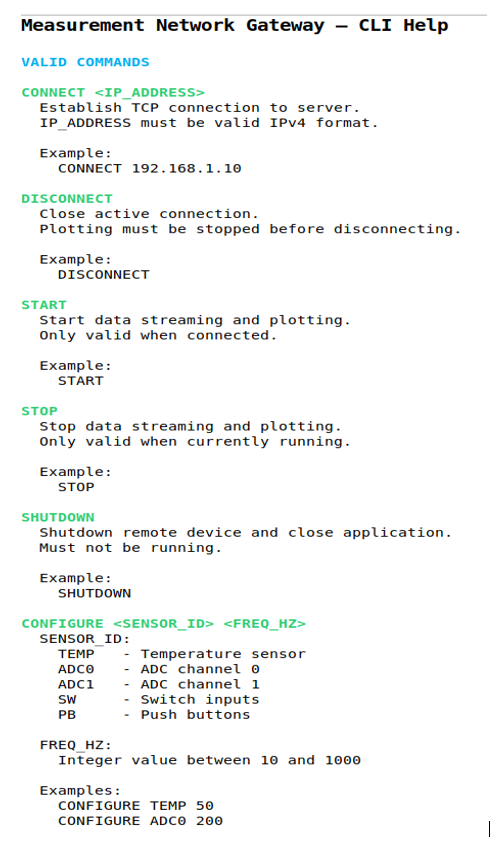
\includegraphics[width = 0.6\textwidth]{media/guihaa10.png}
\label{fig-guihaa10}
\end{figure}

\begin{figure}[H]
\centering 
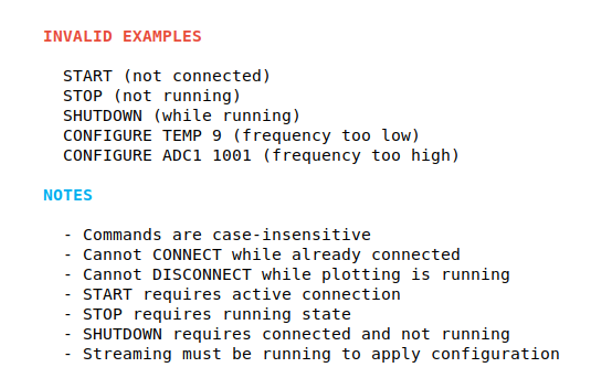
\includegraphics[width = 0.8\textwidth]{media/guihaa11.png}
\label{fig-guihaa11}
\end{figure}

\subsection{SUMMARY}
The plotting subsystem integrates asynchronous data acquisition, synchronized
buffering, and deterministic rendering into a cohesive real-time visualization
framework. Incoming sensor packets are received in a dedicated thread and
inserted into protected circular buffers, ensuring bounded memory usage and
deterministic overwrite behavior. Mutual exclusion guarantees data integrity
during concurrent access, while \texttt{g\_idle\_add} enforces strict
separation between background processing and GTK's main-thread rendering
context. Visualization is performed through a Cairo-based drawing pipeline
within a \texttt{GtkDrawingArea}, refreshed at a controlled interval of
approximately 30 frames per second. A sliding time-window mechanism ensures
that only the most recent and relevant data is displayed, providing a
continuously scrolling view of sensor activity. Samples are normalized to a
unified vertical scale, allowing multiple sensor types to be plotted
simultaneously without dynamic axis reconfiguration. The GUI plot subsystem
further enhances usability through structured grid rendering, dynamic axis
labeling, color-coded multiple sensor traces, and a theme-aware legend. An
auxiliary numerical panel complements the graphical plot by presenting the
latest temperature and ADC values in a bounded textual log. Altogether, the
architecture balances responsiveness, performance stability and clarity of
presentation, resulting in a robust and scalable real-time monitoring
interface.



\clearpage 
\null 
\vfill 
\begin{center}
\textbf{\large Alin Raj Rajagopalan Nair (41520)}
\end{center}
\vfill 
\fancyhead[L]{MNG GUI (Alin Raj Rajagopalan Nair 41520)}
\clearpage


\chapter{MNG GUI Part III}
\section{GUI} 

\subsection{Command Handling}
\begin{enumerate}
    \item \textbf{CONNECT Command}

    Syntax: \texttt{CONNECT <IP\_ADDRESS>}

    \begin{enumerate}
        \item Establishes TCP/IP connection to the remote measurement server on port 50012 using the specified IPv4 address
        \item Implements non-blocking socket creation with 3-second timeout to prevent GUI freezing during connection attempts
        \item Upon successful connection, automatically spawns a dedicated pthread for asynchronous network data reception
        \item Transitions application state from DISCONNECTED to CONNECTED and pre-selects Temperature and ADC1 sensors for immediate visualization
        \item Example: \texttt{CONNECT 192.168.1.10}
    \end{enumerate}

    \item \textbf{DISCONNECT Command}

    Syntax: \texttt{DISCONNECT}

    \begin{itemize}
        \item Gracefully terminates the active TCP connection and stops the network receive thread using \texttt{pthread\_join()} for safe cleanup
        \item Can only be executed when in CONNECTED state; returns error if attempted while streaming is active (must STOP first)
        \item Closes socket file descriptor, clears all sensor circular buffers, and resets timestamp synchronization reference (\texttt{server\_t0})
        \item Transitions application state back to DISCONNECTED, re-enabling the IP entry field and Connect button
        \item Example: \texttt{DISCONNECT}
        \item Error Example: \texttt{DISCONNECT} \\
        \(\rightarrow\) Error: ``Cannot disconnect: GUI is running, stop and disconnect.'' \\
        (when attempted during RUNNING state)
    \end{itemize}

    \item \textbf{START Command}

    Syntax: \texttt{START}

    \begin{itemize}
        \item Sends ASCII \texttt{"START\textbackslash n"} command to the server, initiating real-time binary sensor data streaming over the established TCP connection
        \item Enables sensor selection checkboxes with 2-sensor maximum constraint and activates frequency configuration controls
        \item Transitions state from CONNECTED to RUNNING; disables Disconnect and Shutdown buttons to prevent unsafe operations during streaming
        \item Server responds with initial RATES configuration message followed by continuous batches of \texttt{sensor\_data\_t} structures
        \item Example: \texttt{START}
        \item Typical Workflow Example:
        \begin{enumerate}
            \item \texttt{CONNECT 192.168.1.10}
            \item \texttt{START}
            \item (Data streaming begins, graph updates in real-time)
        \end{enumerate}
    \end{itemize}


    \item \textbf{STOP Command}

    Syntax: \texttt{STOP}

    \begin{itemize}
        \item Sends ASCII \texttt{"STOP\textbackslash n"} command to halt sensor data streaming while maintaining the TCP connection for future operations
        \item Preserves all captured data in circular buffers allowing graph inspection after streaming stops; data persists until disconnect or reconnect
        \item Transitions state from RUNNING to CONNECTED, re-enabling Disconnect and Shutdown buttons while disabling sensor configuration controls
        \item Does not terminate the network receive thread; connection remains active and ready to resume streaming with subsequent START command
        \item Example: \texttt{STOP}
        \item Typical Workflow Example:
        \begin{enumerate}
            \item \texttt{START}
            \item (Observe data for analysis)
            \item \texttt{STOP}
            \item (Graph frozen, data preserved for inspection)
            \item \texttt{START} (can restart streaming)
        \end{enumerate}
    \end{itemize}

    \item \textbf{SHUTDOWN Command}

    Syntax: \texttt{SHUTDOWN}

    \begin{itemize}
        \item Displays modal confirmation dialog before sending \texttt{"SHUTDOWN\textbackslash n"} to the remote embedded device (\texttt{/dev/meascdd}), then exits the application
        \item Automatically sends STOP command first if streaming is active, ensuring clean server-side termination before shutdown
        \item Performs complete cleanup: stops network thread with \texttt{pthread\_join()}, closes socket, clears plot state, and calls \texttt{gtk\_main\_quit()}
        \item Can only be executed from CONNECTED state (not RUNNING); prevents accidental shutdown during active data acquisition
        \item Example: \texttt{SHUTDOWN} \\
        \(\rightarrow\) Dialog: ``Are you sure you want to shutdown the device \texttt{/dev/meascdd}?'' \\
        \(\rightarrow\) User clicks ``Yes'' \(\rightarrow\) Device shuts down, application exits
    \end{itemize}

\end{enumerate}

\textbf{Command Explaination (Detailed)}
\begin{enumerate}
\item The client will send ASCII text commands through the TCP socket connection, which are parsed and executed by the GUI application. Most client commands will be processed based on the command keyword, though some may require additional parameters.
\item Before processing any command, the application will first validate the command syntax and current application state. Only if the command is valid and the state permits execution will it proceed further.
\end{enumerate}

Here are the different commands a client may send:

\begin{enumerate}
    \item \texttt{START} -- Requests data streaming from server.
    \item \texttt{STOP} -- Requests to stop data streaming.
    \item \texttt{CONFIGURE} -- Requests to change a sensor's sampling frequency.
    \item \texttt{DISCONNECT} -- Requests to disconnect from server.
    \item \texttt{SHUTDOWN} -- Requests to shut down the remote device.
    \item \texttt{CONNECT} -- Requests to establish connection with server.
\end{enumerate}

\begin{itemize}
    \item Among these, three commands (\texttt{CONNECT}, \texttt{DISCONNECT},
    \texttt{SHUTDOWN}, \texttt{START}, and \texttt{STOP}) do not require any additional
    parameters. The remaining command (\texttt{CONFIGURE}) requires parameters to
    complete the client's request.
\end{itemize}

\textbf{Client Requesting Data:}
\begin{itemize}
\item In this case, the client is requesting data streaming, specifically the continuous
sensor data from the measurement device. To process this request, the client sends
the ASCII command \texttt{"START\textbackslash n"} to indicate that it wants to begin
receiving real-time sensor data.

\item Once the START command is sent, the server will respond by first transmitting a RATES
message containing the current sampling frequencies for all sensors. This ensures the
client knows the configuration before data streaming begins.

\item After sending the RATES configuration, the server will continuously transmit binary
sensor data batches. Each batch contains multiple \texttt{sensor\_data\_t} structures
(16 bytes each) with \texttt{sensor\_id}, \texttt{sensor\_value}, and \texttt{timestamp}
fields. The network receive thread processes these batches using the \texttt{recv\_all()}
function, which ensures complete message reception by looping until all expected bytes
are received.

\item The received sensor data is inserted into sensor-specific circular buffers protected
by a pthread mutex (\texttt{sample\_lock}). This prevents multiple threads from
accessing the data simultaneously, ensuring data integrity. The GUI continuously
redraws the graph at 33\,ms intervals to display the real-time sensor traces.

\item Here is the example how the client sends the command:
\end{itemize}

\begin{minted}[bgcolor = lightgray, tabsize = 4, breaklines]{c}
// Send START command via TCP socket
send(sock_fd, "START\n", 6, 0);
// Update application state
state = STATE_RUNNING;
\end{minted}

\textbf{Client Requesting to Disable a Sensor:}
\begin{itemize}
\item Similar to a configuration request, the client will disable a sensor through the GUI
by unchecking the sensor's checkbox. This is a client-side operation that does not
send any command to the server.

\item Upon unchecking a checkbox, the application will first validate the 2-sensor maximum
rule by checking whether the total selected sensors exceeds the limit. It will ensure
that users can only display up to 2 sensors simultaneously for optimal visualization.

\item If the checkbox state change is valid, the application will proceed to update the
configuration dropdown and redraw the graph area, effectively removing the sensor's
trace from the display. However, the sensor data continues to be received and stored
in the background circular buffers.

\item Here is the example of how checkbox state affects sensor display:
\end{itemize}
\begin{minted}[bgcolor = lightgray, tabsize = 4, breaklines]{c}
// When user unchecks Temperature checkbox
gtk_toggle_button_set_active(GTK_TOGGLE_BUTTON(checkboxes[0]), FALSE);

// Application updates dropdown
update_dropdown();

// Graph redraws without Temperature trace
gtk_widget_queue_draw(graph_area);
\end{minted}

\textbf{Client Requesting to Enable a Sensor:}
\begin{itemize}
\item Similar to the disable request, the client will enable a sensor by checking the sensor's checkbox. This parameter will specify which sensor the client wants to display on the graph.
\item On the client side, the process will follow the same steps as the disable request. The application will first validate the 2-sensor rule, ensuring that enabling this sensor doesn't exceed the maximum allowed sensors. If the validation passes, the application will proceed with enabling the sensor display.
\item Here is the example of checkbox enabling:
\end{itemize}
\begin{minted}[bgcolor = lightgray, tabsize = 4, breaklines]{c}
// When user checks ADC0 checkbox  
gtk_toggle_button_set_active(GTK_TOGGLE_BUTTON(checkboxes[1]), TRUE);

// Application validates 2-sensor rule and updates display
update_dropdown();
\end{minted}

\textbf{Client Requesting to Change Sample Time of a Sensor:}
\begin{itemize}
\item In this request, the client must send two parameters along with the command. Unlike previous display-only requests, this request requires communication with the server. The client must specify which sensor's sample frequency needs to be changed and the new desired sampling frequency.
\item An important condition to note is that the new sample frequency must be within the range of 10-1000 Hz, which is the valid operating range predefined by the application.
\item On the server side, the process begins with validating the sensor ID, ensuring it falls within the acceptable range (0-4 for the five sensors). In addition to this, the server will also verify the new sample frequency. If the provided sample time is less than 10 Hz or greater than 1000 Hz, the server will reject the request and send an error message back to the client. However, if both conditions are met, the server will proceed with updating the sensor's sampling timer accordingly.

\item Here is the example of client command structure:
\end{itemize}

\begin{minted}[bgcolor = lightgray, tabsize = 4, breaklines]{c}
// Send CONFIGURE command via command line
send(sock_fd, "CONFIGURE TEMP 200\n", strlen("CONFIGURE TEMP 200\n"), 0);

// Or via GUI Configure button
char net_cmd[64];
snprintf(net_cmd, sizeof(net_cmd), "CONFIGURE %s %d\n", "ADC0", 500);
send(sock_fd, net_cmd, strlen(net_cmd), 0);

// Update local frequency table
g_hash_table_replace(sensor_freq, g_strdup("TEMP"), g_strdup("200"));
\end{minted}

\textbf{Client Requesting for Disconnection:}
\begin{itemize}
\item Similar to the START command, the client will send a DISCONNECT command without any parameters. However, instead of requesting data, this command is meant to terminate the connection between the client and the server.
\item Upon receiving this request, the client application will stop the network receive thread and proceed to close the TCP socket connection, effectively disconnecting from the server. The application performs thread cleanup using \texttt{pthread\_join()} to ensure the network thread fully terminates before closing the socket. Once the disconnection is complete, the client will no longer be able to communicate with the server unless a new connection is established.
\item Here is the example of client disconnect implementation:
\end{itemize}
\begin{minted}[bgcolor = lightgray, tabsize = 4, breaklines]{c}
// Stop network thread
if (net_running)
{
      net_running = 0;                                          // Signal thread to exit
      shutdown(sock_fd, SHUT_RDWR);          // Unblock recv() call
      pthread_join(net_thread, NULL);            // Wait for thread termination
}
// Close socket
if (sock_fd >= 0)
{
      close(sock_fd);
      sock_fd = -1;
}
// Reset state
    state = STATE_DISCONNECTED;
\end{minted}

\textbf{Client Requesting for Shutdown:}
\begin{itemize}
\item Similar to other requests without parameters, this command is sent by the client without any additional data. However, unlike a simple disconnection request, this command instructs the server to shut down completely, terminating both the server application and the client GUI.
\item Once the server receives this request, it will first send STOP command if streaming is active, ensuring proper cleanup of sensor data acquisition. After stopping data collection, the server will then proceed to terminate the network thread using \texttt{pthread\_join()}, ensuring that all running threads are properly closed. This step is crucial to prevent any resources from being left open or mismanaged. Once all threads have been successfully terminated, both the client and server will complete the shutdown process and exit the application using \texttt{gtk\_main\_quit()}.
\item Here is the example of client shutdown sequence:
\end{itemize}
\begin{minted}[bgcolor = lightgray, tabsize = 4, breaklines]{c}
// If streaming, stop first
if (state == STATE_RUNNING && sock_fd >= 0)
{
    send(sock_fd, "STOP\n", 5, 0);
}

// Send shutdown command
send(sock_fd, "SHUTDOWN\n", 9, 0);

// Cleanup network resources
if (net_running)
{
    net_running = 0;
    shutdown(sock_fd, SHUT_RDWR);
    pthread_join(net_thread, NULL);
}

// Close socket and exit
close(sock_fd);
gtk_main_quit();
\end{minted}

\subsection{Conclusion}
The Measurement Network Gateway application implements a robust and user-friendly command system that provides dual-interface control through both graphical buttons and a text-based command-line interface. This design philosophy ensures accessibility for users with different preferences while maintaining consistent functionality across both interaction methods.

The command architecture demonstrates several key engineering principles that contribute to reliable embedded systems operation. First, comprehensive state validation ensures that commands can only be executed when the application is in an appropriate state, preventing invalid operations such as attempting to start streaming without an active connection or disconnecting during active data acquisition. This state machine approach (\texttt{DISCONNECTED} $\rightarrow$ \texttt{CONNECTED} $\rightarrow$ \texttt{RUNNING}) provides clear operational boundaries and guides users through proper workflow sequences.

Second, thread-safe communication between the GUI thread and network receive thread is achieved through \texttt{pthread} mutex protection for shared data structures and GTK's \texttt{g\_idle\_add()} mechanism for cross-thread GUI updates. This architecture prevents race conditions and ensures data integrity even during high-frequency sensor streaming at rates up to 1000\,Hz per sensor.

Third, real-time visual feedback enhances user experience by providing immediate confirmation of command execution success or failure. Color-coded borders (green for success, red for errors), dynamic icon changes (terminal $\rightarrow$ checkmark/error $\rightarrow$ terminal), and descriptive status messages inform users about operation outcomes without requiring console output inspection. The automatic timeout-based clearing of feedback messages maintains interface cleanliness while ensuring users receive adequate notification time.

The parameter validation system implements multiple layers of checking: syntax validation ensures correct command format, range validation verifies numerical parameters fall within acceptable bounds (10--1000\,Hz for frequencies, 0--4 for sensor IDs), and state validation confirms operations are permitted in the current application context. Invalid inputs trigger immediate visual feedback and disable action buttons, preventing error-prone operations before they reach the server.

The sensor configuration subsystem demonstrates dynamic UI adaptation, where the dropdown menu automatically rebuilds to reflect only currently displayed sensors, and the frequency entry field auto-populates with stored values when sensor selection changes. The 2-sensor maximum rule is enforced through checkbox sensitivity management, providing intuitive visual feedback (greyed-out checkboxes) that guides user interaction without requiring error dialogs.

The command history system with up/down arrow navigation improves productivity by allowing users to quickly recall and re-execute recent commands, particularly useful during iterative configuration testing. The circular buffer implementation (5 command capacity) stores only successful commands, maintaining a clean history log.

Network communication reliability is ensured through the \texttt{recv\_all()} function, which handles TCP stream fragmentation by looping until complete messages are received, and connection loss detection automatically triggers cleanup callbacks when the server becomes unreachable. The graceful shutdown sequences (\texttt{STOP} $\rightarrow$ \texttt{DISCONNECT} $\rightarrow$ cleanup or \texttt{STOP} $\rightarrow$ \texttt{SHUTDOWN} $\rightarrow$ exit) ensure proper resource release on both client and server sides.

The integration of multiple technologies---GTK+ for GUI rendering, POSIX threads for concurrent network I/O, Cairo for real-time plotting, and BSD sockets for TCP communication---demonstrates modern embedded systems development practices. The separation of concerns (networking in dedicated thread, GUI updates on main thread, data storage in mutex-protected buffers) creates a maintainable and extensible architecture.

Overall, the command system successfully balances ease of use with operational safety, providing both novice users with intuitive graphical controls and experienced users with powerful command-line capabilities. The implementation serves as an effective foundation for professional measurement and data acquisition applications, where reliability, responsiveness, and user experience are paramount.


